\documentclass[
    aspectratio=169, 
    usepdftitle=false, 
    xcolor={dvipsnames},
    hyperref={
        colorlinks,
        linkcolor=black,
        urlcolor=blue}
    ]{beamer}
\usetheme{Madrid}
\usepackage{graphicx}
\usepackage{listings}
\usepackage{soul}

\lstset{
    basicstyle=\ttfamily\footnotesize,
    columns=fullflexible,
    frame=single,
    breaklines=true,
    xleftmargin=10pt,
    xrightmargin=10pt,
}
% \usepackage{xcolor}

\hypersetup{colorlinks,urlcolor=blue}
\addtobeamertemplate{headline}{\hypersetup{linkcolor=.}}{}
\addtobeamertemplate{footline}{\hypersetup{linkcolor=.}}{}

\definecolor{Light}{gray}{.90}
\sethlcolor{Light}

\let\OldTexttt\texttt
\renewcommand{\texttt}[1]{\OldTexttt{\hl{#1}}}% will affect all \texttt

\title[Course Introduction]{Introduction to Python Objects and Expressions}
\subtitle{Lecture 0: Course Introduction}
\author{Daniel Kadyrov}
\date{July 3rd, 2023}

\begin{document}

\begin{frame}
\titlepage
\end{frame}

\begin{frame}{Agenda}
    \tableofcontents
\end{frame}

\section{Course and Instructor Introduction}
\begin{frame}{About me}
    \framesubtitle{Early Life}
    \begin{itemize}
    \item Born and raised in New York City
    \begin{itemize}
        \item Grew up in Murray Hill, Manhattan
        \item Went to PS 116, Salk School of Science, and Nest+M
        \item Currently living in Harlem with my dog Karl Marx
    \end{itemize}
    \item Hobbies include chess, bike commuting, yoga, and surfing
    \item Social causes I care about include bicycle and transportation infrastructure, clean water access, and hearing loss awareness
    \end{itemize}
\end{frame}

\begin{frame}{About me}
    \framesubtitle{Higher Education}
    \begin{itemize}
        \item SUNY Binghamton University
        \begin{itemize}
            \item 2015 Bachelor of Science: Mechanical Engineering
            \item 2016 Master of Science: Mechanical Engineering (Acoustics \& Dynamic Systems)
            \item Clubs: WHRW Radio Station, MIDI, Engineering without Borders
        \end{itemize}
        \item Stevens Institute of Technology
        \begin{itemize}
            \item 2021 Master of Science: Computer Science (Data Analysis \& Machine Learning)
            \item 2024 Ph.D. Ocean Engineering
        \end{itemize}
    \end{itemize}
\end{frame}

\begin{frame}{About me}
    \framesubtitle{Work Experience}
    \begin{itemize}
        \item Engineering Experience: 
        \begin{itemize}
            \item 2017-2018: Senior Engineer at Thornton Tomasetti
            \item 2019-Present: Research Engineer at the STAR Center
        \end{itemize}
        \item Teaching Experience: Tutoring, ScholarStem, Chess at Three, Eleanor Roosavelt STEM Course
        \item Other Experience: 
        \begin{itemize} 
            \item Food Service: Sigmund's Pretzel Shop, Ray's Candy Store
            \item Music: Live/Recording Engineering, DJing, cocktail jazz piano
            \item Other: REI SoHo, Lifeguard
        \end{itemize}
    \end{itemize}
\end{frame}

\section{Group Introduction}
\begin{frame}{Group Introduction}
    \framesubtitle{Group Survey}

    \begin{columns}
        \begin{column}{0.5\textwidth}
            \begin{block}{Fill out this survey}
                \url{https://forms.gle/VM3yhQr4FZrhaCXz6}
            \end{block}
        \end{column}
        \begin{column}{0.5\textwidth}  %%<--- here
            \begin{center}
             
\includegraphics[width=0.5\textwidth]{qr-code.pdf}
             \end{center}
        \end{column}
    \end{columns}
\end{frame}

\begin{frame}{Course Information}
    \framesubtitle{Learning Objectives}
    \begin{itemize}
        \item Learn the basics of Python programming including data structures, functions, and classes while utilizing industry standard programs and packages to develop, test, debug, and collaborate on projects
        \item Set the foundations of using Python for data science applications including:
        \begin{itemize}
            \item Collecting, parsing, sanitizing and cleaning, standardizing, and exploring datasets
            \item Generating visualizations including graphics, tables, and figures
            \item Determine trends and report conclusions from analysis
        \end{itemize}
    \end{itemize}
\end{frame}

\begin{frame}{Course Information}
    \framesubtitle{Assignments}
    \begin{itemize}
        \item Daily assignments on the materials we learned in class. Most likely you will work on these assignments through the end of class and submit them at the beginning at the beginning of the next class
        \item There will be a final project that will be presented at the end of the semester that will be a culmination of the skills we learned in class
    \end{itemize}
\end{frame}

\begin{frame}{Course Information}
    \framesubtitle{Office Hours and Contact Information}
    \begin{itemize}
        \item Office hours will be by appointment only
        \item Contact email: daniel.kadyrov@gmail.com
    \end{itemize}
\end{frame}

\section{Course Downloads}
\begin{frame}{Course Downloads}
\begin{enumerate}
    \item Git and GitHub
    \item Python through PyEnv
    \item Visual Studio Code
\end{enumerate}
\end{frame}

\begin{frame}{GitHub}
    \framesubtitle{Create a GitHub student account}

    GitHub offers free accounts to students. It comes with unlimited public repositories and unlimited collaborators as well as other perks. You will need to verify your student status.

    \begin{columns}
        \begin{column}{0.5\textwidth}
            \begin{block}{Sign up here}
                \url{https://education.github.com/}
            \end{block}
        \end{column}
        \begin{column}{0.5\textwidth}  %%<--- here
            \begin{center}
             
\includegraphics[width=0.5\textwidth]{qr-code.pdf}
             \end{center}
        \end{column}
    \end{columns}
\end{frame}

\begin{frame}{GitHub}
    \framesubtitle{Download and install Git}

    Git is a way to manage your code and collaborate with others. It is a version control system that allows you to track changes to your code and revert back to previous versions if necessary. It also allows you to collaborate with others on the same code base.

    \begin{columns}
        \begin{column}{0.5\textwidth}
            \begin{block}{Download Git here}
                \url{https://git-scm.com/downloads}
            \end{block}
        \end{column}
        \begin{column}{0.5\textwidth}  %%<--- here
            \begin{center}
             
\includegraphics[width=0.5\textwidth]{qr-code.pdf}
             \end{center}
        \end{column}
    \end{columns}
\end{frame}

\begin{frame}{GitHub}
    \framesubtitle{Course Repository}

    The coursework, including all documents, assignments, and code will be hosted on GitHub. You will need to fork the repository to your own GitHub account. This will allow you to make changes to the code without affecting the original code. You will also be able to download the code, through cloning, to your local machine.

    \begin{block}{Course Repository}
        \url{https://github.com/dkadyrov/introductiontopython}
    \end{block}
    
\end{frame}

\begin{frame}[fragile]{GitHub}
    \framesubtitle{Fork and clone the repository}

    To fork the repository, go to the repository in your browser and click the fork button in the top right corner. This will create a copy of the repository in your GitHub account. To clone the repository, go to the repository in your browser and click the green code button. Copy the link.\\~\

    In terminal, you can navigate to the directory you want to clone the repository to through the \texttt{cd} command. Then, type \texttt{git clone <link>} where \texttt{<link>} is the link you copied from the repository. This will create a copy of the repository on your local machine. This is demonstrated in the following code block:

    \begin{lstlisting}
cd Documents
cd "Columbia Summer Course"
git clone <link>
    \end{lstlisting}
\end{frame}

\begin{frame}{Python}
    \framesubtitle{Installing Pyenv}
    Python has many different distributions, versions, and management tools. Although Anaconda is commonly used for data science, we will be using \href{https://github.com/pyenv/pyenv}{PyEnv} to manage our Python distributions.\\~\

    Python constantly gets updated. Currently it is on version 3.11.3. However, many packages and programs still use older versions of Python. PyEnv allows us to manage multiple versions of Python on our machine. We can also set a default version of Python to use.\\
\end{frame}

\begin{frame}[fragile]{Python}
    \framesubtitle{Installing Pyenv}

    \begin{block}{Windows OS}
        Copy and paste the following code into your Command Prompt:
        \begin{lstlisting}
Invoke-WebRequest -UseBasicParsing -Uri "https://raw.githubusercontent.com/pyenv-win/pyenv-win/master/pyenv-win/install-pyenv-win.ps1" -OutFile "./install-pyenv-win.ps1"; &"./install-pyenv-win.ps1"
        \end{lstlisting}
    \end{block}

    \begin{block}{Mac OS}
        Copy and paste the following code into your Terminal:
        \begin{lstlisting}
alias brew='env PATH="${PATH//$(pyenv root)\/shims:/}" brew'
        \end{lstlisting}
    \end{block}

\end{frame}

\begin{frame}[fragile]{Python}
    \framesubtitle{Checking for PyEnv}

    To check that PyEnv was installed correctly, type \texttt{pyenv} into your terminal or command prompt. You should see a list of commands that you can use with PyEnv.

    \begin{center}
        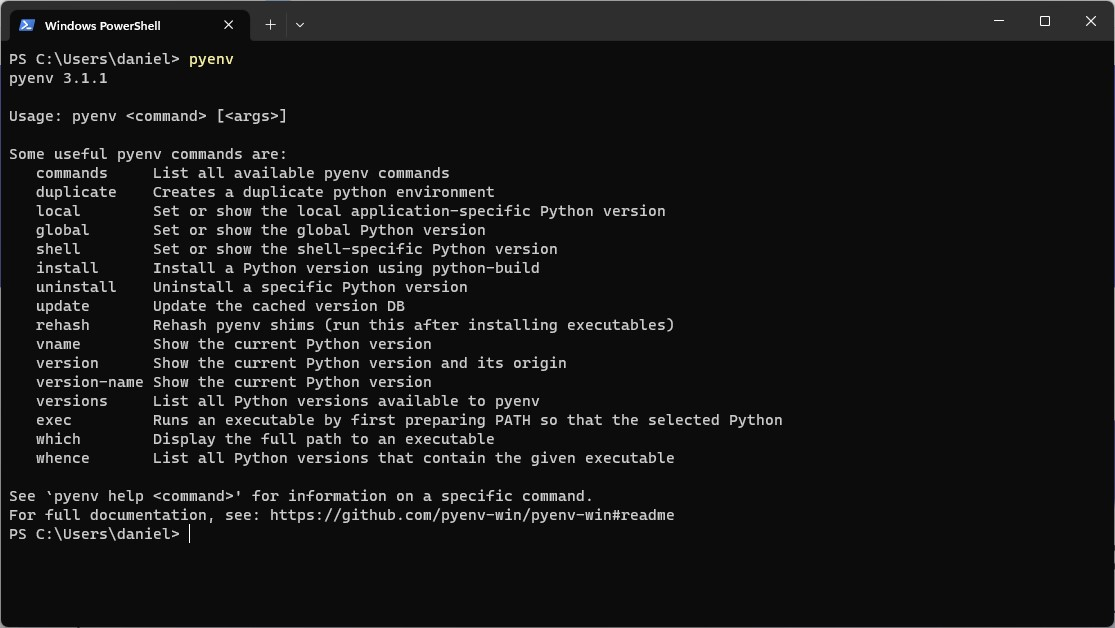
\includegraphics[width=0.5\textwidth]{pyenv_terminal.jpg}
    \end{center}

    If you do not see this, try restarting your terminal or command prompt. If you still do not see this, you will have to add PyEnv to your PATH.
\end{frame}

\begin{frame}[fragile]{Python}
    \framesubtitle{Installing Python through PyEnv}

    To install Python through PyEnv, type \texttt{pyenv install <version>} where \texttt{<version>} is the version of Python you want to install. For example, to install Python 3.8.5, type \texttt{pyenv install 3.8.5}. This environment now needs to be set as the global, default, Python environment through the \texttt{global} command. This course is going to use Python 3.10.10 as its distribution.\\~\

    \begin{lstlisting}
pyenv install 3.10.10
pyenv global 3.10.10
    \end{lstlisting}
\end{frame}

\begin{frame}{Visual Studio Code}
    \begin{enumerate}
        \item Download and install \href{https://code.visualstudio.com/download}{Visual Studio Code}
        \item Install the Python extension
        \item Choose your theme! 
    \end{enumerate}
\end{frame}

\end{document}